%% ============================================================
%% Paper02_WD_Aspirations.tex
%% Developing Educational and Vocational Aspirations through
%% International Child Sponsorship: Evidence from Kenya,
%% Indonesia, and Mexico
%% Ross, Glewwe, Prudencio, Wydick -- World Development (2021)
%%
%% Compile: cd Slides
%%   TEXINPUTS=../Preambles:$TEXINPUTS xelatex -interaction=nonstopmode Paper02_WD_Aspirations.tex
%%   BIBINPUTS=..:$BIBINPUTS bibtex Paper02_WD_Aspirations
%%   TEXINPUTS=../Preambles:$TEXINPUTS xelatex -interaction=nonstopmode Paper02_WD_Aspirations.tex
%%   TEXINPUTS=../Preambles:$TEXINPUTS xelatex -interaction=nonstopmode Paper02_WD_Aspirations.tex
%% ============================================================
\documentclass[aspectratio=169, 10pt]{beamer}
%% ============================================================
%% header.tex -- Shared Beamer preamble for Research Portfolio
%% Compile with: XeLaTeX (3-pass + bibtex)
%% Colors match Quarto/emory-clean.scss for cross-format consistency
%% ============================================================

%% ---- Packages -----------------------------------------------
\usepackage{fontspec}           % XeLaTeX font loading
\usepackage{unicode-math}       % Unicode math support
\usepackage{amsmath, mathtools} % Math environments
\usepackage{booktabs}           % Publication-quality tables
\usepackage{multirow}           % Multi-row table cells
\usepackage{graphicx}           % Include figures
\usepackage{xcolor}             % Color definitions
\usepackage{tcolorbox}          % Colored boxes
\tcbuselibrary{skins, breakable}
\usepackage{natbib}             % Author-year citations
\usepackage{appendixnumberbeamer} % Appendix slides don't count in total
\usepackage{hyperref}           % Hyperlinks
\usepackage{tikz}               % Diagrams (if needed)

%% ---- Fonts --------------------------------------------------
%% Using TeX Gyre Heros (Helvetica-style, bundled with MiKTeX).
%% To switch to Source Sans Pro: install it, then swap the two blocks below.
\setmainfont{TeX Gyre Heros}
\setsansfont{TeX Gyre Heros}
% Alternative: uncomment below and comment above if Source Sans Pro is installed
% \setmainfont{Source Sans Pro}[BoldFont=Source Sans Pro SemiBold]
% \setsansfont{Source Sans Pro}[BoldFont=Source Sans Pro SemiBold]

%% ---- Colors (matching emory-clean.scss) ---------------------
\definecolor{navyblue}{HTML}{012169}
\definecolor{institutgold}{HTML}{2E75B6}   % steel blue (was gold #B9975B)
\definecolor{highlightyellow}{HTML}{F2A900}
\definecolor{lightbg}{HTML}{E8EDF5}
\definecolor{darkgray}{HTML}{1a1a1a}
\definecolor{medgray}{HTML}{555555}
\definecolor{lightgray}{HTML}{f8f9fa}
\definecolor{positivegreen}{HTML}{15803d}
\definecolor{negativered}{HTML}{b91c1c}

%% ---- Beamer Theme -------------------------------------------
\usetheme{default}
\usecolortheme{default}
\setbeamertemplate{navigation symbols}{}   % No navigation clutter

%% Frame title
\setbeamercolor{frametitle}{fg=white, bg=navyblue}
\setbeamertemplate{frametitle}{%
  \vspace*{0.3em}%
  \insertframetitle%
  \vspace*{0.3em}%
}
\setbeamerfont{frametitle}{series=\bfseries, size=\large}

%% Title page colors
\setbeamercolor{title}{fg=navyblue}
\setbeamercolor{subtitle}{fg=institutgold}
\setbeamercolor{author}{fg=navyblue}
\setbeamercolor{institute}{fg=medgray}
\setbeamercolor{date}{fg=institutgold}

%% Body
\setbeamercolor{background canvas}{bg=white}
\setbeamercolor{normal text}{fg=darkgray}
\setbeamerfont{normal text}{family=\sffamily}

%% Itemize bullets
\setbeamercolor{item}{fg=navyblue}
\setbeamercolor{subitem}{fg=institutgold}
\setbeamertemplate{itemize item}{\small\textbullet}
\setbeamertemplate{itemize subitem}{\small$\rightarrow$}

%% Block environments
\setbeamercolor{block title}{fg=white, bg=navyblue}
\setbeamercolor{block body}{fg=darkgray, bg=lightbg}
\setbeamercolor{block title alerted}{fg=white, bg=institutgold}
\setbeamercolor{block body alerted}{fg=darkgray, bg=white}

%% Footer
\setbeamertemplate{footline}{%
  \hfill%
  \usebeamerfont{page number in head/foot}%
  \usebeamercolor[fg]{page number in head/foot}%
  \insertframenumber\,/\,\inserttotalframenumber\kern1em%
  \vskip4pt%
}
\setbeamercolor{page number in head/foot}{fg=medgray}

%% Section slides (automatically centered, navy bg)
\AtBeginSection[]{%
  \begin{frame}[plain]
    \begin{tikzpicture}[remember picture, overlay]
      \fill[navyblue] (current page.south west) rectangle (current page.north east);
      \node[white, font=\bfseries\Large, align=center] at (current page.center)
        {\insertsectionhead};
    \end{tikzpicture}
  \end{frame}%
}

%% ---- Custom Box Environments --------------------------------

%% keybox: gold background, for key takeaways
\newtcolorbox{keybox}{%
  colback=institutgold!12!white,
  colframe=institutgold,
  leftrule=4pt, rightrule=0pt, toprule=0pt, bottomrule=0pt,
  arc=4pt, outer arc=4pt,
  boxsep=2pt, left=6pt, right=6pt, top=5pt, bottom=5pt,
}

%% methodbox: navy left bar, for model/identification
\newtcolorbox{methodbox}{%
  colback=navyblue!5!white,
  colframe=navyblue,
  leftrule=4pt, rightrule=0pt, toprule=0pt, bottomrule=0pt,
  arc=4pt, outer arc=4pt,
  boxsep=2pt, left=6pt, right=6pt, top=5pt, bottom=5pt,
}

%% resultbox: gold border, for main findings
\newtcolorbox{resultbox}{%
  colback=institutgold!10!white,
  colframe=institutgold,
  leftrule=2pt, rightrule=2pt, toprule=2pt, bottomrule=2pt,
  arc=4pt, outer arc=4pt,
  boxsep=2pt, left=6pt, right=6pt, top=5pt, bottom=5pt,
}

%% assumptionbox: titled, formal assumptions
\newtcolorbox{assumptionbox}[1][]{%
  colback=highlightyellow!8!white,
  colframe=highlightyellow!70!black,
  leftrule=2pt, rightrule=2pt, toprule=2pt, bottomrule=2pt,
  arc=4pt, outer arc=4pt,
  boxsep=2pt, left=6pt, right=6pt, top=5pt, bottom=5pt,
  title={#1},
  fonttitle=\bfseries\small,
  attach boxed title to top left={yshift=-2mm, xshift=6pt},
  boxed title style={colback=highlightyellow!70!black, arc=2pt},
}

%% ---- Convenience Commands -----------------------------------
\newcommand{\gold}[1]{{\color{institutgold}\textbf{#1}}}
\newcommand{\navy}[1]{{\color{navyblue}\textbf{#1}}}
\newcommand{\pos}[1]{{\color{positivegreen}\textbf{#1}}}
\newcommand{\bad}[1]{{\color{negativered}\textbf{#1}}}   % red annotation
\newcommand{\hi}[1]{{\color{navyblue}\textbf{#1}}}
% Note: \alert is Beamer built-in (styled gold via alerted text color below)
\setbeamercolor{alerted text}{fg=institutgold}

%% ---- Math shortcuts -----------------------------------------
\newcommand{\E}{\mathbb{E}}
\newcommand{\Prob}{\mathbb{P}}
\newcommand{\ATE}{\mathrm{ATE}}
\newcommand{\ATT}{\mathrm{ATT}}
\newcommand{\MTE}{\mathrm{MTE}}
\newcommand{\Norm}{\mathcal{N}}


%% ---- Bibliography -------------------------------------------
\bibliographystyle{aer}
\setcitestyle{authoryear, open={(}, close={)}}

%% ============================================================
\begin{document}

%% ---- 1. Title Slide -----------------------------------------
\begin{frame}[plain]
  \vspace{1.5em}
  \begin{center}
    {\color{navyblue}\Large\bfseries
      Developing Educational and Vocational Aspirations\\[0.3em]
      through International Child Sponsorship:\\[0.3em]
      Evidence from Kenya, Indonesia, and Mexico}\\[1em]
    {\color{institutgold}\large\itshape World Development 140 (2021)}\\[1.5em]
    {\color{navyblue}\normalsize\bfseries
      Phillip H.\ Ross \quad Paul Glewwe \quad Daniel Prudencio \quad Bruce Wydick}\\[0.3em]
    {\color{medgray}\small Analysis Group \,/\, U.\ Minnesota \,/\, Rice University \,/\, U.\ San Francisco}\\[1.5em]
    {\color{institutgold}\small Published: November 2020}
  \end{center}
\end{frame}

%% ---- 2. Roadmap ---------------------------------------------
\begin{frame}{Roadmap}
  \tableofcontents
\end{frame}

%% ============================================================
\section{Motivation \& Research Question}
%% ============================================================

%% ---- 3. The Big Question ------------------------------------
\begin{frame}{Child Sponsorship: Beyond Material Inputs}
  \begin{columns}
    \begin{column}{0.55\textwidth}
      \textbf{Child sponsorship programs} transfer resources from wealthy sponsors to children in developing countries:
      \begin{itemize}
        \item School fees, uniforms, nutritious meals, healthcare
        \item Monthly contribution: \$25--40; avg.\ duration: 9 years
        \item Compassion International: $>$2 million children, 25 countries
      \end{itemize}
      \vspace{0.7em}
      Prior work (\citealt{Wydick2013, Wydick2017}) finds \gold{large adult life impacts}: schooling, employment, income.

      \vspace{0.7em}
      \textbf{The open question:} sponsorship programs also invest heavily in \navy{socio-emotional development} --- self-esteem, optimism, aspirations. Does this matter?
    \end{column}
    \begin{column}{0.41\textwidth}
      \begin{keybox}
        \textbf{This paper asks:}\\[0.4em]
        Does Compassion International's child sponsorship program increase \gold{self-esteem}, \gold{optimism}, and \gold{educational/vocational aspirations} among sponsored children?\\[0.5em]
        And do these psychological gains \gold{mediate} the program's effects on schooling?
      \end{keybox}
    \end{column}
  \end{columns}
\end{frame}

%% ---- 4. Aspirations & Poverty Traps (TikZ) -----------------
\begin{frame}{Internal Constraints and Poverty Traps}
  \begin{columns}
    \begin{column}{0.50\textwidth}
      A growing theoretical literature shows that \navy{low aspirations} can sustain poverty independently of material constraints:
      \begin{itemize}
        \item \citealt{Ray2006}: aspirations failures create self-reinforcing traps
        \item \citealt{Genicot2017}: aspirations and inequality diverge in equilibrium
        \item \citealt{Lybbert2018}: relaxing \emph{both} internal and external constraints may be necessary
      \end{itemize}
      \vspace{0.5em}
      Interventions that raise aspirations can break the cycle --- but \bad{causal evidence is scarce}.
    \end{column}
    \begin{column}{0.46\textwidth}
      \begin{center}
      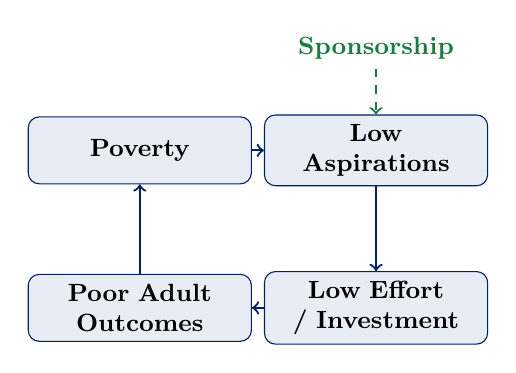
\begin{tikzpicture}[
          box/.style={rectangle, rounded corners=4pt, draw=navyblue, fill=lightbg,
                      text width=2.6cm, align=center, font=\small\bfseries,
                      minimum height=0.85cm},
          arr/.style={->, thick, navyblue},
          brkarr/.style={->, thick, positivegreen, dashed}
        ]
        \node[box] (pov) at (0,  1.1) {Poverty};
        \node[box] (asp) at (3,  1.1) {Low\\Aspirations};
        \node[box] (eff) at (3, -0.9) {Low Effort\\/ Investment};
        \node[box] (out) at (0, -0.9) {Poor Adult\\Outcomes};

        \draw[arr] (pov.east)  -- (asp.west);
        \draw[arr] (asp.south) -- (eff.north);
        \draw[arr] (eff.west)  -- (out.east);
        \draw[arr] (out.north) -- (pov.south);

        % Intervention
        \node[font=\small\color{positivegreen}\bfseries] (ci) at (3, 2.4) {Sponsorship};
        \draw[brkarr] (ci) -- (asp.north);
      \end{tikzpicture}
      \end{center}
      \vspace{0.2em}
      {\small \color{medgray} Sponsorship breaks the trap by raising aspirations directly.}
    \end{column}
  \end{columns}
\end{frame}

%% ---- 5. What We Already Know --------------------------------
\begin{frame}{What We Already Know: Large Adult Impacts}
  \begin{columns}
    \begin{column}{0.55\textwidth}
      \citealt{Wydick2013} study 9,144 adults across 6 countries who were sponsored as children:
      \begin{itemize}
        \item \pos{+12--18 pp} increase in secondary school completion (baseline: 44.5\%)
        \item \pos{+6.6 pp} probability of white-collar employment
        \item \pos{+\$13--17/month} income over a \$75 baseline
      \end{itemize}
      \vspace{0.5em}
      \citealt{Wydick2017}: sponsorship effects on income and wealth persist into adulthood.
      \vspace{0.5em}
      These are \gold{large relative to other celebrated interventions} (e.g., Progresa CCT: +0.66 years of education).
    \end{column}
    \begin{column}{0.41\textwidth}
      \begin{methodbox}
        \textbf{Why is the effect so large?}\\[0.4em]
        Standard explanations (fees, uniforms, meals) are \emph{also} provided by Progresa --- yet Compassion's effects are $2\times$ larger.\\[0.5em]
        \textbf{Hypothesis:} Non-pecuniary inputs --- self-esteem, optimism, and aspirations --- are part of the answer.
      \end{methodbox}
    \end{column}
  \end{columns}
\end{frame}

%% ---- 6. The Knowledge Gap ----------------------------------
\begin{frame}{The Knowledge Gap: Mechanisms Are Unclear}
  \begin{columns}
    \begin{column}{0.55\textwidth}
      Despite strong reduced-form evidence on adult outcomes, \bad{the psychological channel has not been credibly identified}:
      \begin{itemize}
        \item No multi-country study of sponsorship effects on psychology
        \item No causal identification of aspirations effects with plausible exogenous variation
        \item No mediation analysis linking psychological gains to schooling outcomes
      \end{itemize}
      \vspace{0.5em}
      \textbf{Companion paper:} \citealt{Glewwe2018} use children's self-portraits in Indonesia to measure hopefulness --- suggestive but single-country and qualitative.
    \end{column}
    \begin{column}{0.41\textwidth}
      \begin{keybox}
        \textbf{This paper fills the gap:}\\[0.4em]
        1. \gold{Multi-country} causal evidence on psychology\\[0.3em]
        2. \gold{Age-eligibility IV} for exogenous sponsorship\\[0.3em]
        3. \gold{Mediation analysis} linking aspirations to grade completion
      \end{keybox}
    \end{column}
  \end{columns}
\end{frame}

%% ---- 7. Research Questions ----------------------------------
\begin{frame}{Research Questions \& Preview of Findings}
  \begin{columns}
    \begin{column}{0.55\textwidth}
      \textbf{Three questions:}
      \begin{enumerate}
        \item Does sponsorship increase \navy{self-esteem}, \navy{optimism}, and \navy{aspirations} among currently sponsored children?
        \item Does it increase \navy{grade completion}?
        \item Do psychological gains \navy{mediate} the schooling effect?
      \end{enumerate}
      \vspace{0.7em}
      \textbf{Sample:} 2,022 children in Kenya, Indonesia, and Mexico
    \end{column}
    \begin{column}{0.41\textwidth}
      \begin{resultbox}
        \textbf{Preview of main findings:}\\[0.4em]
        Sponsorship increases self-esteem \gold{(+0.25$\sigma$)}, optimism \gold{(+0.26$\sigma$)}, and aspirations \gold{(+0.29$\sigma$)}\\[0.3em]
        Grade completion: \gold{+0.56 years}\\[0.3em]
        Aspirations mediate \gold{$\approx$10\%} of the schooling effect
      \end{resultbox}
    \end{column}
  \end{columns}
\end{frame}

%% ============================================================
\section{Contribution to the Literature}
%% ============================================================

%% ---- 8. Strand 1: Development Traps & Aspirations ----------
\begin{frame}{Literature: Development Traps and Internal Constraints}
  \begin{columns}
    \begin{column}{0.55\textwidth}
      \textbf{Theoretical foundations:}
      \begin{itemize}
        \item \citealt{Ray2006}: aspirations as a reference point in utility --- convex below, concave above; failures create poverty traps
        \item \citealt{Dalton2016}: poverty reduces cognitive bandwidth for setting aspirations
        \item \citealt{Genicot2017}: aspirations and inequality: divergence vs.\ convergence equilibria
        \item \citealt{Lybbert2018}: model of aspirations windows --- relaxing \emph{both} constraints matters
      \end{itemize}
    \end{column}
    \begin{column}{0.41\textwidth}
      \begin{keybox}
        \textbf{Common theme:}\\[0.4em]
        Internal constraints (aspirations, self-efficacy, hope) can trap the poor as effectively as external constraints (credit, access).\\[0.5em]
        Programs that address \emph{both} may be transformative.
      \end{keybox}
    \end{column}
  \end{columns}
\end{frame}

%% ---- 9. Strand 2: Psychology in Development Economics -------
\begin{frame}{Literature: Psychology and Development}
  \begin{columns}
    \begin{column}{0.55\textwidth}
      \textbf{Empirical evidence on psychological interventions:}
      \begin{itemize}
        \item \citealt{Benabou2003}: encouragement raises self-esteem $\to$ academic achievement
        \item \citealt{Laajaj2017}: pessimism about the future $\to$ shortened planning horizon; savings intervention expands it
        \item \citealt{Baranov2020}: maternal depression treatment raises children's human capital investments
      \end{itemize}
      \vspace{0.5em}
      General finding: psychological interventions have positive but \gold{heterogeneous} impacts (\citealt{Anderson2008} indices help address multiple testing).
    \end{column}
    \begin{column}{0.41\textwidth}
      \begin{methodbox}
        \textbf{Methodological challenge:}\\[0.4em]
        Most studies use single-country data, lack credible instruments, or focus on adults.\\[0.5em]
        We study \emph{currently sponsored children} with a sharp age-based instrument across \emph{three countries}.
      \end{methodbox}
    \end{column}
  \end{columns}
\end{frame}

%% ---- 11. Our Contribution -----------------------------------
\begin{frame}{Our Contribution}
  \begin{columns}
    \begin{column}{0.55\textwidth}
      \textbf{Three innovations relative to existing work:}
      \vspace{0.4em}
      \begin{enumerate}
        \item \navy{Multi-country causal identification}: IV based on program age-eligibility rule in Kenya, Indonesia, and Mexico simultaneously
        \vspace{0.3em}
        \item \navy{Psychological outcomes}: direct measurement of self-esteem, optimism, and educational/vocational aspirations using validated scales
        \vspace{0.3em}
        \item \navy{Mediation analysis}: formal test of whether psychological gains mediate observed schooling effects
      \end{enumerate}
    \end{column}
    \begin{column}{0.41\textwidth}
      \begin{resultbox}
        \textbf{Policy relevance:}\\[0.4em]
        If aspirations mediate adult outcome effects, then program design should \gold{explicitly prioritize} socio-emotional skill development --- not just material inputs.\\[0.5em]
        Sponsorship programs transfer $\approx$\$3.4 billion/year to children in developing countries \citep{Wydick2013}.
      \end{resultbox}
    \end{column}
  \end{columns}
\end{frame}

%% ============================================================
\section{Institutional Background \& Data}
%% ============================================================

%% ---- 12. Compassion International --------------------------
\begin{frame}{Compassion International: What the Program Does}
  \begin{columns}
    \begin{column}{0.50\textwidth}
      \textbf{Program features:}
      \begin{itemize}
        \item Faith-based Christian organization; $>$2M children in 25 countries
        \item Monthly sponsorship $\approx$ \$25--40; program lasts $\approx$9 years on average
        \item Weekly tutoring/child development: 4--8 hours, 48 weeks/year
        \item Child--sponsor relationship: letters, photos, gifts
      \end{itemize}
      \vspace{0.4em}
      \textbf{Key feature:} Unlike CCTs, Compassion emphasizes \navy{holistic child development} --- the non-pecuniary components are as central as the material ones.
    \end{column}
    \begin{column}{0.46\textwidth}
      \begin{center}
      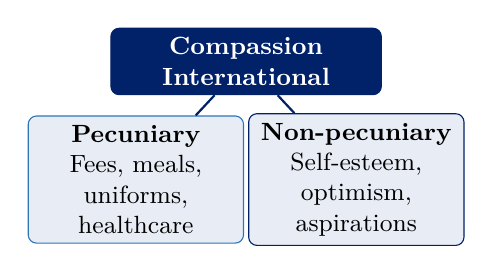
\begin{tikzpicture}[
          level 1/.style={sibling distance=2.8cm},
          every node/.style={rectangle, rounded corners=3pt, font=\small,
                             text width=2.5cm, align=center, minimum height=0.7cm},
          edge from parent/.style={draw, thick, navyblue}
        ]
        \node[draw=navyblue, fill=navyblue, text=white, font=\small\bfseries,
              text width=3.2cm] {Compassion\\International}
          child { node[draw=institutgold, fill=lightbg] {\textbf{Pecuniary}\\Fees, meals,\\uniforms,\\healthcare} }
          child { node[draw=navyblue, fill=lightbg] {\textbf{Non-pecuniary}\\Self-esteem,\\optimism,\\aspirations} };
      \end{tikzpicture}
      \end{center}
      \vspace{0.2em}
      {\small \color{medgray} This paper focuses on the \textbf{non-pecuniary} branch.}
    \end{column}
  \end{columns}
\end{frame}

%% ---- 13. Study Design & Countries --------------------------
\begin{frame}{Study Design: Three Countries}
  \begin{center}
  \small
  \begin{tabular}{lp{3.8cm}p{2.4cm}cc}
    \toprule
    \textbf{Country} & \textbf{Treatment sites} & \textbf{Control} & \textbf{N} & \textbf{Fieldwork} \\
    \midrule
    Kenya     & Rironi, Isinya, Njoro                & Siblings            & 570  & May--Jul 2011 \\
    Indonesia & Jakarta, 4 sites                    & Waitlist HH         & 526  & May--Jul 2012 \\
    Mexico    & 4 villages, Oaxaca \& Chiapas        & Neighboring villages & 926 & Jun--Jul 2017 \\
    \midrule
    \textbf{Total} & & & \textbf{2,022} & \\
    \bottomrule
  \end{tabular}
  \end{center}
  \vspace{0.5em}
  \begin{columns}
    \begin{column}{0.55\textwidth}
      \begin{itemize}
        \item Sites selected to exploit the \navy{age-eligibility rule}: children $\leq$9 years old at program rollout were eligible
        \item Surveys conducted by university students unaffiliated with Compassion
      \end{itemize}
    \end{column}
    \begin{column}{0.41\textwidth}
      \begin{methodbox}
        \textbf{Cross-country differences:}\\[0.3em]
        Kenya: siblings only as controls\\
        Indonesia: waitlist households\\
        Mexico: neighboring villages\\[0.3em]
        $\Rightarrow$ IV absorbs these differences
      \end{methodbox}
    \end{column}
  \end{columns}
\end{frame}

%% ---- 14. Sample Construction --------------------------------
\begin{frame}{Sample Construction: Who Was Surveyed}
  \begin{center}
  \begin{tabular}{lp{6cm}c}
    \toprule
    \textbf{Group} & \textbf{Description} & \textbf{N (pooled)} \\
    \midrule
    Sponsored children    & Currently enrolled in Compassion program & 956 \\
    Non-sponsored siblings & Next oldest/youngest sibling in same household & varies \\
    Waitlist households   & On Compassion waitlist (Indonesia) & 79 \\
    Control villages      & Neighboring communities without program (Mexico) & 217 \\
    \bottomrule
  \end{tabular}
  \end{center}
  \vspace{0.4em}
  \begin{columns}
    \begin{column}{0.55\textwidth}
      \begin{itemize}
        \item Age range: 10--18 at survey (Kenya); 8--18 (Indonesia); 10--18 (Mexico)
        \item Limit per household: 1 (Kenya), 2 (Indonesia), 3 (Mexico)
        \item Interviews conducted away from parents, teachers, and Compassion staff
      \end{itemize}
    \end{column}
    \begin{column}{0.41\textwidth}
      \begin{methodbox}
        \textbf{Key design choice:}\\[0.3em]
        Comparison groups chosen to address \emph{all three} endogeneity concerns (community, household, within-household selection)
      \end{methodbox}
    \end{column}
  \end{columns}
\end{frame}

%% ---- 15. Outcome Variables ----------------------------------
\begin{frame}{Outcome Variables: Three Indices + Schooling}
  \begin{columns}
    \begin{column}{0.55\textwidth}
      \textbf{Three summary indices} (Anderson 2008 methodology):
      \begin{itemize}
        \item \navy{Self-esteem index}: Rosenberg (1965) 10-item scale; demean + normalize within community
        \item \navy{Optimism index}: General Social Survey items on future hopefulness and optimism
        \item \navy{Aspirations index}: Composite of hope/expectation for white-collar job + years of education expected
      \end{itemize}
      \vspace{0.4em}
      \textbf{Schooling outcome:}
      \begin{itemize}
        \item \navy{Grade completion}: years of education completed at time of survey
      \end{itemize}
    \end{column}
    \begin{column}{0.41\textwidth}
      \begin{methodbox}
        \textbf{Why summary indices?}\\[0.3em]
        Multiple outcomes $\Rightarrow$ multiple testing problem. Anderson (2008) indices:
        \begin{itemize}\small
          \item Weight by inverse covariance
          \item Reduce false discovery rate
          \item Provide concise test of ``general effect''
        \end{itemize}
        \vspace{0.2em}
        FDR $q$-values reported for all results.
      \end{methodbox}
    \end{column}
  \end{columns}
\end{frame}

%% ---- 16. Summary Statistics ---------------------------------
\begin{frame}{Summary Statistics: Sponsored vs.\ Non-Sponsored}
  \begin{center}
  \small
  \begin{tabular}{lcccc}
    \toprule
    & \textbf{All} & \textbf{Sponsored} & \textbf{Non-Sponsored} & \textbf{Difference} \\
    \midrule
    Self-Esteem Index  & $-$0.002 & 0.032  & $-$0.036 & 0.068 \\
    Optimism Index     & $-$0.000 & 0.080  & $-$0.080 & 0.160$^{***}$ \\
    Hope: White-collar (\%) & 71.5 & 69.4 & 73.5 & 0.042$^{**}$ \\
    Expect: White-collar (\%) & 67.5 & 69.0 & 66.1 & 0.029 \\
    Years of Education Exp.\ & 14.92 & 15.13 & 14.71 & 0.419$^{***}$ \\
    Aspirations Index  & $-$0.001 & 0.068  & $-$0.060 & 0.136$^{***}$ \\
    Age                & 12.62 & 12.17 & 13.07 & $-$0.902$^{***}$ \\
    Father: White-collar & 18.9\% & 20.8\% & 17.1\% & 0.037$^{**}$ \\
    \midrule
    Observations       & 2,022 & 956 & 1,066 & \\
    \bottomrule
  \end{tabular}
  \end{center}
  \vspace{0.2em}
  {\small \color{medgray} Sponsored children are younger ($-$0.9 years) and from households where fathers are more likely to have white-collar jobs --- motivating the IV strategy.}
\end{frame}

%% ============================================================
\section{Empirical Strategy}
%% ============================================================

%% ---- 17. Three Sources of Endogeneity (TikZ DAG) -----------
\begin{frame}{Three Sources of Endogeneity}
  \begin{columns}
    \begin{column}{0.50\textwidth}
      Comparing sponsored to non-sponsored children is \bad{not} straightforward. Three potential biases:
      \begin{enumerate}
        \item \navy{Community selection}: Compassion targets needier communities $\Rightarrow$ treatment communities differ on observables
        \item \navy{Household selection}: Compassion targets neediest households within communities $\Rightarrow$ biases toward zero
        \item \navy{Within-household selection}: Parents choose the ``neediest'' child $\Rightarrow$ downward bias on intra-household estimates
      \end{enumerate}
    \end{column}
    \begin{column}{0.46\textwidth}
      \begin{center}
      \scalebox{0.82}{%
      \begin{tikzpicture}[
          source/.style={ellipse, draw=navyblue, fill=lightbg, font=\small\bfseries,
                         text width=2cm, align=center, minimum height=0.8cm},
          treat/.style={ellipse, draw=institutgold, fill=institutgold!20,
                        font=\small\bfseries, text width=2cm, align=center,
                        minimum height=0.8cm},
          iv/.style={rectangle, rounded corners=3pt, draw=positivegreen,
                     fill=white, font=\small\bfseries, text width=2.0cm, align=center,
                     minimum height=0.7cm},
          arr/.style={->, thick, navyblue},
          ivarr/.style={->, thick, positivegreen, dashed}
        ]
        % Source nodes (left column)
        \node[source] (com) at (0, 2.8)  {Community};
        \node[source] (hh)  at (0, 1.4)  {Household};
        \node[source] (ch)  at (0, 0)    {Child};
        % Treatment node (right)
        \node[treat]  (sp)  at (3.5, 1.4) {Sponsorship};
        % IV node (below child, bottom-left)
        \node[iv]     (iv)  at (0, -1.3) {Age at\\Rollout (IV)};

        % Bias arrows (fan from left to right)
        \draw[arr] (com.east) to[out=0,  in=130] (sp.north west);
        \draw[arr] (hh.east)  --  (sp.west);
        \draw[arr] (ch.east)  to[out=0, in=230] (sp.south west);

        % IV arrow curves below child to reach Sponsorship cleanly
        \draw[ivarr] (iv.east) to[out=0, in=270] (sp.south);
      \end{tikzpicture}}
      \end{center}
      {\small \color{medgray} The IV provides exogenous variation in sponsorship,\\bypassing all three selection biases.}
    \end{column}
  \end{columns}
\end{frame}

%% ---- 18. The Age-Eligibility Rule ---------------------------
\begin{frame}{Identification: The Age-Eligibility Rule}
  \begin{columns}
    \begin{column}{0.55\textwidth}
      \textbf{Key institutional feature:} Children had to be \navy{$\leq$9 years old} when a Compassion program was introduced in their community to be eligible for sponsorship.

      \vspace{0.6em}
      This creates exogenous variation \emph{within households}:
      \begin{itemize}
        \item Older siblings (age $>$9 at rollout): ineligible $\Rightarrow$ low sponsorship probability
        \item Younger siblings (age $\leq$9 at rollout): eligible $\Rightarrow$ high sponsorship probability
      \end{itemize}
      \vspace{0.5em}
      \textbf{Instruments:} Dummies for child's age at time of program rollout (ages $-3$ to $+9$; excluded group: age $\geq 10$)
    \end{column}
    \begin{column}{0.41\textwidth}
      \begin{assumptionbox}[Exclusion Restriction]
        Age at program rollout affects psychological outcomes \emph{only} through its effect on sponsorship status --- not through direct age effects on psychology, conditional on controls.\\[0.4em]
        Controls include: current age, gender, birth order, household FE.
      \end{assumptionbox}
    \end{column}
  \end{columns}
\end{frame}

%% ---- 19. The Discontinuity (figure placeholder) ------------
\begin{frame}{The Discontinuity: First-Stage Intuition}
  \begin{columns}
    \begin{column}{0.55\textwidth}
      \begin{center}
        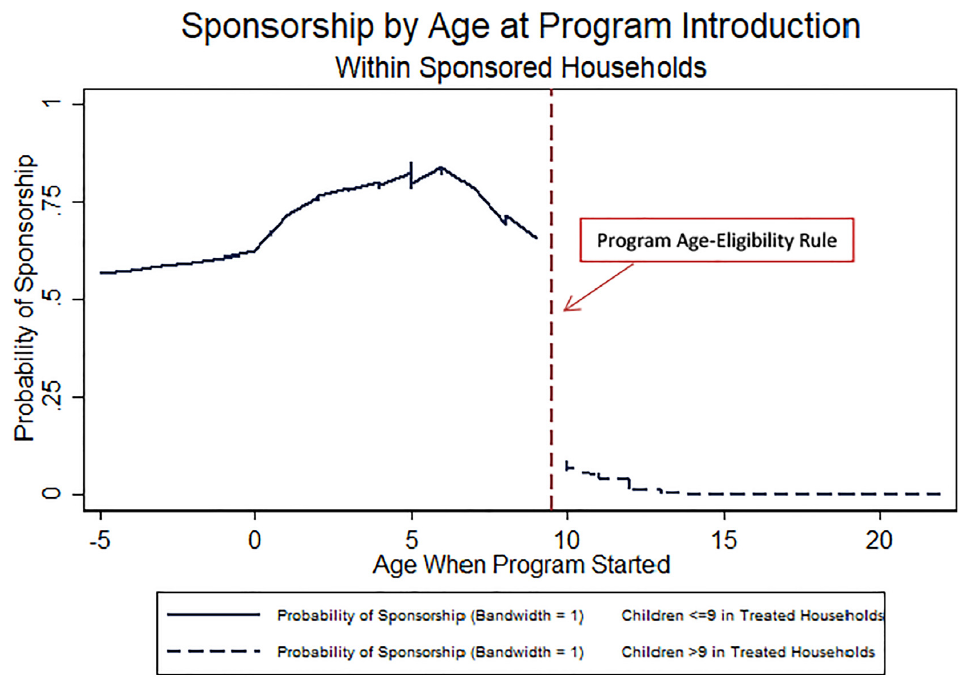
\includegraphics[width=\textwidth]{../Figures/fig1_discontinuity}
      \end{center}
    \end{column}
    \begin{column}{0.41\textwidth}
      \textbf{Reading the figure:}
      \begin{itemize}
        \item X-axis: child's age when program started
        \item Y-axis: probability of being sponsored (bandwidth = 1)
        \item \navy{Solid line}: children in treated households, age $\leq$9 at rollout
        \item \navy{Dashed line}: children in treated households, age $>$9 at rollout
      \end{itemize}
    \end{column}
  \end{columns}
\end{frame}

%% ---- 20. First-Stage Equations ------------------------------
\begin{frame}{Econometric Specification: First Stage}
  \begin{columns}
    \begin{column}{0.55\textwidth}
      \textbf{First stage} (community fixed effects):
      \[
        T_i = \alpha_v + \boldsymbol{\varphi}'\mathbf{X}_{ij} + \lambda'\mathbf{Z}_i + \delta C_j + \gamma S_j + u_{ijv}
      \]

      \textbf{First stage} (household fixed effects):
      \[
        T_i = \alpha_j + \boldsymbol{\varphi}'\mathbf{X}_i + \lambda'\mathbf{Z}_i + u_{ijv}
      \]

      \vspace{0.5em}
      where $\mathbf{Z}_i$ = vector of \navy{age-at-rollout dummies} (ages $-3$ to $+9$), the excluded instruments.
    \end{column}
    \begin{column}{0.41\textwidth}
      \begin{methodbox}
        \textbf{Key controls:}\\[0.3em]
        $\mathbf{X}_{ij}$: age, gender, birth order, dwelling quality, parental occupation\\[0.3em]
        $C_j$: dummy for sponsored household (Indonesia, Mexico)\\[0.3em]
        $S_j$: dummy for sponsored village (Mexico)\\[0.3em]
        $\alpha_j$: household FE (preferred spec.) --- absorbs all between-household differences
      \end{methodbox}
    \end{column}
  \end{columns}
\end{frame}

%% ---- 21. Second-Stage Equations -----------------------------
\begin{frame}{Econometric Specification: Second Stage}
  \begin{columns}
    \begin{column}{0.55\textwidth}
      \textbf{Second stage} (community FE):
      \[
        y_{ijv} = \alpha_v + \gamma\widehat{T}_i + \boldsymbol{\beta}'\mathbf{X}_{ij} + \pi C_j + \delta S_j + e_{ijv}
      \]

      \textbf{Second stage} (household FE):
      \[
        y_{ijv} = \alpha_j + \gamma\widehat{T}_i + \boldsymbol{\beta}'\mathbf{X}_i + e_{ijv}
      \]

      \vspace{0.4em}
      where $\widehat{T}_i$ = instrumented probability of sponsorship.

      \vspace{0.4em}
      \textbf{Preferred specification:} household FE + demographic controls (Panel D in results tables)
    \end{column}
    \begin{column}{0.41\textwidth}
      \begin{methodbox}
        \textbf{Estimation notes:}\\[0.3em]
        Standard errors clustered at household level.\\[0.3em]
        Equal country weights in pooled estimations.\\[0.3em]
        FDR $q$-values (Anderson 2008) for the 3 summary indices to correct for multiple testing.
      \end{methodbox}
    \end{column}
  \end{columns}
\end{frame}

%% ---- 22. First-Stage Results --------------------------------
\begin{frame}{First-Stage Results: Strong Instrument Relevance}
  \begin{center}
  \small
  \begin{tabular}{lcccc}
    \toprule
    & \textbf{Kenya} & \textbf{Indonesia} & \textbf{Mexico} & \textbf{Pooled} \\
    \midrule
    Age at rollout dummies & \multicolumn{4}{c}{(coefficients for ages 3--9 all positive and significant)} \\[0.3em]
    Households & 207 & 259 & 236 & 703 \\
    Observations & 455 & 518 & 531 & 1,506 \\
    \midrule
    \textbf{F-statistic (instruments)} & \textbf{75.38} & \textbf{28.43} & \textbf{8.07} & \textbf{36.73} \\
    \bottomrule
  \end{tabular}
  \end{center}
  \vspace{0.4em}
  \begin{columns}
    \begin{column}{0.55\textwidth}
      \begin{itemize}
        \item Age-at-rollout dummies strongly predict sponsorship across all countries
        \item Kenya: strongest first stage (F = 75); Mexico: weakest but adequate (F = 8)
      \end{itemize}
    \end{column}
    \begin{column}{0.41\textwidth}
      \begin{keybox}
        Children who were $\leq$9 years old when the program arrived are substantially more likely to be sponsored than their older siblings --- as expected from the eligibility rule.
      \end{keybox}
    \end{column}
  \end{columns}
\end{frame}

%% ============================================================
\section{Pooled Results}
%% ============================================================

%% ---- 23. Headline Summary ----------------------------------
\begin{frame}{Pooled Results: Headline Summary}
  \begin{columns}
    \begin{column}{0.55\textwidth}
      \textbf{Preferred specification:} 2SLS with household fixed effects + demographic controls (Panel D, Table 8).

      \vspace{0.5em}
      Sponsorship has \gold{positive and statistically significant} causal effects on:
      \begin{itemize}
        \item Self-esteem: \pos{+0.255$\sigma$} ($p < 0.05$)
        \item Optimism: \pos{+0.259$\sigma$} ($p < 0.05$)
        \item Aspirations index: \pos{+0.292$\sigma$} ($p < 0.05$)
        \item Grade completion: \pos{+0.56 years} ($p < 0.01$)
      \end{itemize}
      \vspace{0.4em}
      All six 2SLS estimates in Panel D are \navy{positive}; three are significant at $p < 0.05$.
    \end{column}
    \begin{column}{0.41\textwidth}
      \begin{resultbox}
        \textbf{Key result:}\\[0.4em]
        Sponsorship significantly raises children's psychological well-being and aspirations, with effects consistent across multiple specifications and index construction methods.\\[0.5em]
        These effects are \gold{larger in 2SLS than OLS}, consistent with negative within-household selection.
      \end{resultbox}
    \end{column}
  \end{columns}
\end{frame}

%% ---- 24. Self-Esteem & Optimism ----------------------------
\begin{frame}{Pooled Results: Self-Esteem and Optimism}
  \begin{center}
  \small
  \begin{tabular}{lcccc}
    \toprule
    & \multicolumn{2}{c}{\textbf{Self-Esteem Index}} & \multicolumn{2}{c}{\textbf{Optimism Index}} \\
    \cmidrule(lr){2-3} \cmidrule(lr){4-5}
    & OLS & 2SLS & OLS & 2SLS \\
    \midrule
    Panel A: Community FE, No Controls    & 0.043 & $-$0.235$^{**}$ & 0.087 & 0.018 \\
    Panel B: Community FE + Controls      & 0.112$^{**}$ & 0.041 & 0.159$^{***}$ & 0.348$^{***}$ \\
    Panel C: Household FE, No Controls   & 0.068 & 0.084 & 0.008 & 0.051 \\
    \textbf{Panel D: HH FE + Controls}   & \textbf{0.108}$^{*}$ & \textbf{0.255}$^{**}$ & \textbf{0.053} & \textbf{0.259}$^{**}$ \\
    \midrule
    Households (Panel D) & 533 & 697 & 533 & 697 \\
    \bottomrule
  \end{tabular}
  \end{center}
  \vspace{0.3em}
  \begin{columns}
    \begin{column}{0.55\textwidth}
      \begin{itemize}
        \item 2SLS $>$ OLS in preferred spec: consistent with Compassion targeting neediest children (downward OLS bias)
      \end{itemize}
    \end{column}
    \begin{column}{0.41\textwidth}
      \begin{methodbox}
        \small FDR $q$-values (Panel D):\\
        Self-esteem: $q = 0.021$\\
        Optimism: $q = 0.021$\\[0.3em]
        Robust to multiple testing.
      \end{methodbox}
    \end{column}
  \end{columns}
\end{frame}

%% ---- 25. Aspirations ---------------------------------------
\begin{frame}{Pooled Results: Aspirations}
  \begin{center}
  \small
  \begin{tabular}{lcc}
    \toprule
    & \textbf{OLS} & \textbf{2SLS} \\
    \midrule
    Panel A: Community FE, No Controls     & 0.139$^{**}$ & 0.387$^{***}$ \\
    Panel B: Community FE + Controls       & 0.107$^{*}$  & 0.466$^{***}$ \\
    Panel C: Household FE, No Controls    & 0.125$^{**}$ & 0.279$^{**}$  \\
    \textbf{Panel D: HH FE + Controls}    & \textbf{0.102} & \textbf{0.292}$^{**}$ \\
    \bottomrule
  \end{tabular}
  \end{center}
  \vspace{0.4em}
  \begin{columns}
    \begin{column}{0.55\textwidth}
      \begin{itemize}
        \item Aspirations show the \gold{most consistent} positive effects across all 8 panels (all positive, 7 of 8 statistically significant)
        \item FDR $q = 0.005$ in Panel B; $q = 0.261$ in preferred Panel D (less precise within-HH)
        \item Component indices: hope and expectation for white-collar job both positive but smaller and less significant
      \end{itemize}
    \end{column}
    \begin{column}{0.41\textwidth}
      \begin{keybox}
        Aspirations is the \gold{most robustly affected} psychological dimension.\\[0.4em]
        Children under Compassion's care develop stronger goals for education and career --- the key input to the mediation story.
      \end{keybox}
    \end{column}
  \end{columns}
\end{frame}

%% ---- 26. Grade Completion ----------------------------------
\begin{frame}{Pooled Results: Grade Completion}
  \begin{center}
  \small
  \begin{tabular}{lcccc}
    \toprule
    & \multicolumn{2}{c}{\textbf{OLS}} & \multicolumn{2}{c}{\textbf{2SLS}} \\
    \cmidrule(lr){2-3} \cmidrule(lr){4-5}
    & Comm.\ FE & HH FE & Comm.\ FE & HH FE \\
    \midrule
    No additional controls     & 0.332$^{***}$ & 0.282$^{***}$ & 0.526$^{***}$ & 0.564$^{***}$ \\
    With demographic controls  & 0.286$^{***}$ & 0.300$^{***}$ & 0.555$^{***}$ & 0.567$^{***}$ \\
    \midrule
    Households (HH FE + controls) & \multicolumn{2}{c}{534} & \multicolumn{2}{c}{698} \\
    \bottomrule
  \end{tabular}
  \end{center}
  \vspace{0.3em}
  \begin{columns}
    \begin{column}{0.55\textwidth}
      \begin{itemize}
        \item 2SLS: sponsorship increases grade completion by \pos{0.56 years} (preferred spec.)
        \item Effect consistent across all 8 specifications ($p < 0.01$ throughout)
        \item Smaller than adult retrospective estimates in \citealt{Wydick2013} (1.03--1.46 years) --- children still enrolled
      \end{itemize}
    \end{column}
    \begin{column}{0.41\textwidth}
      \begin{resultbox}
        Sponsorship \gold{raises current grade completion by 0.56 years} among children still in the program --- a meaningful early-life effect consistent with aspirations-driven effort.
      \end{resultbox}
    \end{column}
  \end{columns}
\end{frame}

%% ---- 27. Results Summary Table -----------------------------
\begin{frame}{Pooled Results: Summary of Preferred 2SLS Estimates}
  \begin{center}
  \small
  \begin{tabular}{lccc}
    \toprule
    \textbf{Outcome} & \textbf{Estimate} & \textbf{Std.\ Error} & \textbf{Significance} \\
    \midrule
    Self-Esteem Index       & +0.255$\sigma$ & (0.110) & $p < 0.05$ \\
    Optimism Index          & +0.259$\sigma$ & (0.109) & $p < 0.05$ \\
    Hope: White-collar (\%) & +0.077         & (0.048) & $p < 0.10$ \\
    Expect: White-collar (\%)& +0.046        & (0.052) & n.s. \\
    Education Expected (yrs) & +0.437        & (0.236) & $p < 0.10$ \\
    Aspirations Index       & +0.292$\sigma$ & (0.119) & $p < 0.05$ \\
    \midrule
    Grade Completion (yrs)  & +0.567         & (0.131) & $p < 0.01$ \\
    \bottomrule
  \end{tabular}
  \end{center}
  \vspace{0.2em}
  {\small \color{medgray} Preferred specification: 2SLS, household fixed effects, demographic controls (Panel D). Standard errors clustered at household level.}
  \vspace{0.3em}
  \begin{keybox}
    \small Sponsorship produces broad, positive psychological effects. All point estimates are positive --- the combination of uniformly positive estimates with multiple significant results provides strong evidence of a general program effect on child well-being.
  \end{keybox}
\end{frame}

%% ============================================================
\section{Heterogeneity by Country}
%% ============================================================

%% ---- 28. Kenya Results ------------------------------------
\begin{frame}{Country Results: Kenya}
  \begin{columns}
    \begin{column}{0.55\textwidth}
      \textbf{2SLS, household FE + controls (Table 6, Panel A):}
      \begin{itemize}
        \item Self-Esteem: \pos{+0.336$\sigma^{***}$}
        \item Optimism: $-$0.001 (n.s.)
        \item Hope for white-collar: \pos{+0.114 pp$^{***}$}
        \item Grade completion: \pos{+0.555 years$^{***}$}
        \item Aspirations Index: \pos{+0.368$\sigma^{***}$}
      \end{itemize}
      \vspace{0.4em}
      \textbf{Strongest effects} of all three countries. Self-esteem and aspirations both significant at $q < 0.01$.
    \end{column}
    \begin{column}{0.41\textwidth}
      \begin{keybox}
        \textbf{Why Kenya?}\\[0.4em]
        Kenya has the most challenging baseline conditions: lower education, worse employment, lower income. \citealt{Wydick2013} find larger adult impacts in Sub-Saharan Africa too.\\[0.4em]
        Internal constraints may matter \emph{more} when external conditions are worse.
      \end{keybox}
    \end{column}
  \end{columns}
\end{frame}

%% ---- 29. Indonesia Results ---------------------------------
\begin{frame}{Country Results: Indonesia}
  \begin{columns}
    \begin{column}{0.55\textwidth}
      \textbf{2SLS, household FE + controls (Table 6, Panel B):}
      \begin{itemize}
        \item Self-Esteem: +0.138 (n.s.)
        \item Optimism: \pos{+0.512$\sigma^{***}$}
        \item Hope for white-collar: +0.057 (n.s.)
        \item Grade completion: +0.529 years ($p < 0.01$)
        \item Aspirations Index: +0.225 (n.s.)
      \end{itemize}
      \vspace{0.4em}
      Optimism is the standout effect. Self-esteem and aspirations positive but imprecisely estimated.
    \end{column}
    \begin{column}{0.41\textwidth}
      \begin{methodbox}
        \textbf{Note on Indonesia sample:}\\[0.3em]
        Includes non-sponsored children from \emph{waitlist} households (needier than random comparison group) $\Rightarrow$ comparison group is already disadvantaged $\Rightarrow$ may compress effect estimates.\\[0.3em]
        Robustness: restricting to 1--2 child households yields similar results.
      \end{methodbox}
    \end{column}
  \end{columns}
\end{frame}

%% ---- 30. Mexico Results ------------------------------------
\begin{frame}{Country Results: Mexico}
  \begin{columns}
    \begin{column}{0.55\textwidth}
      \textbf{2SLS, household FE + controls (Table 6, Panel C):}
      \begin{itemize}
        \item Self-Esteem: $-$0.004 (n.s.)
        \item Optimism: $-$0.280 (n.s.)
        \item Hope for white-collar: $-$0.102 (n.s.)
        \item Grade completion: \pos{+1.539 years} (large but SE = 1.035)
        \item Aspirations Index: +0.402 (n.s.)
      \end{itemize}
      \vspace{0.4em}
      Point estimates generally positive (except optimism), but \bad{statistically insignificant} throughout due to large standard errors.
    \end{column}
    \begin{column}{0.41\textwidth}
      \begin{methodbox}
        \textbf{Why imprecise in Mexico?}\\[0.4em]
        Lowest F-statistic (8.07) $\Rightarrow$ weaker first stage.\\[0.3em]
        Shortest average sponsorship duration (3.98 years vs.\ 7.0 in Kenya) $\Rightarrow$ smaller exposure.\\[0.3em]
        Comparison: non-sponsored from \emph{neighboring} villages (not same household).
      \end{methodbox}
    \end{column}
  \end{columns}
\end{frame}

%% ---- 31. Why Heterogeneity? --------------------------------
\begin{frame}{Understanding Cross-Country Heterogeneity}
  \begin{columns}
    \begin{column}{0.55\textwidth}
      \textbf{Three contributing factors:}
      \vspace{0.3em}
      \begin{enumerate}
        \item \navy{Counterfactual conditions}: Effects larger where baseline conditions are worse (Kenya $>$ Indonesia $>$ Mexico). Consistent with a ``room to grow'' in aspirations.

        \vspace{0.3em}
        \item \navy{Years of sponsorship}: Kenya 7.0 yrs, Indonesia 7.3 yrs, Mexico 3.98 yrs. Longer exposure $\Rightarrow$ stronger effects.

        \vspace{0.3em}
        \item \navy{Precision}: Kenya has the strongest first stage (F = 75) and tightest within-household comparisons.
      \end{enumerate}
    \end{column}
    \begin{column}{0.41\textwidth}
      \begin{keybox}
        \textbf{Broader lesson:}\\[0.4em]
        Child sponsorship's psychological impact is \gold{context-dependent}: it matters more where children face greater internal and external constraints at baseline.\\[0.5em]
        This is consistent with \citealt{Wydick2013}, who find the largest adult impacts in Sub-Saharan Africa.
      \end{keybox}
    \end{column}
  \end{columns}
\end{frame}

%% ============================================================
\section{Mediation Analysis}
%% ============================================================

%% ---- 32. Why Mediation Matters (TikZ path diagram) ---------
\begin{frame}{Mediation: Does Psychology Drive Schooling Gains?}
  \begin{columns}
    \begin{column}{0.50\textwidth}
      We know sponsorship raises:
      \begin{itemize}
        \item Psychological indices (self-esteem, optimism, aspirations)
        \item Grade completion (+0.56 years)
      \end{itemize}
      \vspace{0.4em}
      \textbf{Key question:} do the psychological gains \emph{causally explain} the schooling gains?
      \vspace{0.4em}

      If aspirations rise, children may:
      \begin{itemize}
        \item Study harder (effort channel)
        \item Stay in school longer (dropout reduction)
        \item Self-select into higher grades (aspiration-congruent behavior)
      \end{itemize}
    \end{column}
    \begin{column}{0.46\textwidth}
      \begin{center}
      \scalebox{0.78}{%
      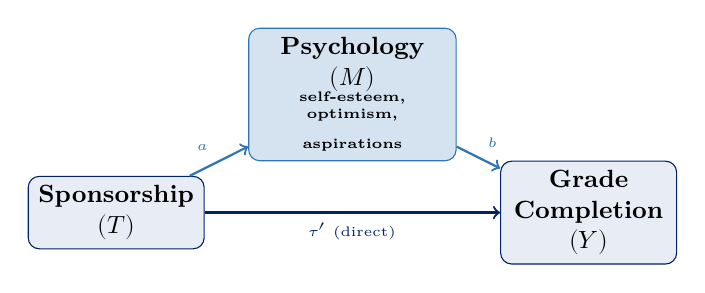
\begin{tikzpicture}[
          box/.style={rectangle, rounded corners=4pt, draw=navyblue, fill=lightbg,
                      font=\small\bfseries, text width=2.0cm, align=center,
                      minimum height=0.85cm},
          med/.style={rectangle, rounded corners=4pt, draw=institutgold, fill=institutgold!20,
                      font=\small\bfseries, text width=2.4cm, align=center,
                      minimum height=0.85cm},
          arr/.style={->, thick, navyblue},
          marr/.style={->, thick, institutgold}
        ]
        \node[box] (T) at (0,0)   {Sponsorship\\$(T)$};
        \node[med] (M) at (3,1.5) {Psychology\\$(M)$\\{\tiny self-esteem, optimism,\\aspirations}};
        \node[box] (Y) at (6,0)   {Grade\\Completion\\$(Y)$};

        \draw[marr] (T) -- (M) node[midway, above left, font=\tiny\color{institutgold}] {$a$};
        \draw[marr] (M) -- (Y) node[midway, above right, font=\tiny\color{institutgold}] {$b$};
        \draw[arr]  (T) -- (Y) node[midway, below, font=\tiny\color{navyblue}] {$\tau'$ (direct)};
      \end{tikzpicture}}
      \end{center}
      \vspace{0.3em}
      {\small Indirect: $a \times b$ \quad Total: $\tau = \tau' + a \times b$}
    \end{column}
  \end{columns}
\end{frame}

%% ---- 33. Mediation Framework --------------------------------
\begin{frame}{Mediation Framework: Econometric Setup}
  \begin{columns}
    \begin{column}{0.55\textwidth}
      \textbf{Baron \& Kenny (1986) / Preacher \& Hayes (2008) framework:}

      \vspace{0.4em}
      Three estimating equations:
      \[
        Y = \tau_0 + \tau T + \varepsilon_R \quad \text{(reduced form)}
      \]
      \[
        M = a_0 + aT + \varepsilon_M \quad \text{(mediator equation)}
      \]
      \[
        Y = b_0 + bM + cT + \varepsilon_Y \quad \text{(outcome equation)}
      \]
      Indirect effect: $a \times b$; standard errors via bootstrapping.
    \end{column}
    \begin{column}{0.41\textwidth}
      \begin{assumptionbox}[Key Endogeneity Concern]
        $M$ may be correlated with $\varepsilon_Y$ (e.g., parental support for schooling raises both aspirations and grades).\\[0.4em]
        If $\mathrm{Cov}(M, \varepsilon_Y) > 0$: estimate of $b$ is \emph{upward biased}.\\[0.4em]
        $\Rightarrow$ Our $a \times b$ is an \gold{upper bound} on the mediated effect.\\[0.3em]
        We interpret significance of $a \times b$ as a \emph{necessary condition} for mediation.
      \end{assumptionbox}
    \end{column}
  \end{columns}
\end{frame}

%% ---- 34. Mediation Results ----------------------------------
\begin{frame}{Mediation Results}
  \begin{center}
  \small
  \begin{tabular}{lccc}
    \toprule
    \textbf{Mediator} & \textbf{Point Est.\ ($a \times b$)} & \textbf{CI 90\%} & \textbf{CI 95\%} \\
    \midrule
    \multicolumn{4}{l}{\textit{Panel A: OLS}} \\
    Aspirations  & 0.0258 & [0.0002,\ 0.0544] & [$-$0.0046,\ 0.0608] \\
    Self-esteem  & 0.0114 & [0.0003,\ 0.0270] & [$-$0.0009,\ 0.0311] \\
    Optimism     & 0.0062 & [$-$0.0014,\ 0.0184] & [$-$0.0029,\ 0.0219] \\
    \midrule
    \multicolumn{4}{l}{\textit{Panel B: 2SLS}} \\
    Aspirations  & 0.0543 & [0.0097,\ 0.1054] & [0.0020,\ 0.1173] \\
    Self-esteem  & 0.0202 & [0.0008,\ 0.0480] & [$-$0.0013,\ 0.0554] \\
    Optimism     & 0.0151 & [$-$0.0029,\ 0.0405] & [$-$0.0063,\ 0.0480] \\
    \bottomrule
  \end{tabular}
  \end{center}
  \vspace{0.2em}
  {\small \color{medgray} Confidence intervals from bootstrap (data quartiles). Total 2SLS effect on grade completion: 0.567 years.}
  \begin{columns}
    \begin{column}{0.55\textwidth}
      \begin{itemize}
        \item \gold{Aspirations}: mediates $\approx$10\% of total effect ($p < 0.05$, 2SLS)
        \item \gold{Self-esteem}: mediates $\approx$5\% ($p < 0.10$, 2SLS)
        \item Optimism: positive but insignificant
      \end{itemize}
    \end{column}
    \begin{column}{0.41\textwidth}
      \begin{keybox}
        \small Aspirations are the \gold{primary psychological channel} linking sponsorship to schooling outcomes.
      \end{keybox}
    \end{column}
  \end{columns}
\end{frame}

%% ---- 35. Bootstrap Distributions (figure placeholder) ------
\begin{frame}{Bootstrap Distributions of Mediation Estimates (2SLS)}
  \begin{columns}[t]
    \begin{column}{0.31\textwidth}
      \begin{center}
        
\includegraphics[width=\textwidth]{{../Figures/Fig 2A}}\\[0.3em]
        {\small \textbf{Self-Esteem}}\\
        {\tiny 90\% CI excludes 0}
      \end{center}
    \end{column}
    \begin{column}{0.31\textwidth}
      \begin{center}
        
\includegraphics[width=\textwidth]{{../Figures/Fig 2B}}\\[0.3em]
        {\small \textbf{Optimism}}\\
        {\tiny CI straddles 0 --- not significant}
      \end{center}
    \end{column}
    \begin{column}{0.31\textwidth}
      \begin{center}
        
\includegraphics[width=\textwidth]{{../Figures/Fig 2C}}\\[0.3em]
        {\small \textbf{Aspirations}}\\
        {\tiny \gold{90\% \& 95\% CI both exclude 0}}
      \end{center}
    \end{column}
  \end{columns}
  \vspace{0.4em}
  {\small \color{medgray} Bootstrap confidence intervals (data quartiles). Aspirations is the primary mediating channel.
  Imai et al.\ (2011) method yields similar results.}
\end{frame}

%% ============================================================
\section{Robustness}
%% ============================================================

%% ---- 36. Robustness 1: Alternative Index -------------------
\begin{frame}{Robustness: Alternative Index Construction}
  \textbf{Panel A of Table 11:} Replace Anderson (2008) indices with Kling, Liebman \& Katz (2007) equal-weight indices.

  \vspace{0.8em}
  \begin{columns}[c]
    \begin{column}{0.48\textwidth}
      Results (2SLS, HH FE + controls, pooled):
      \begin{itemize}
        \item Self-Esteem: \pos{+0.243$\sigma^{**}$}
        \item Optimism: \pos{+0.283$\sigma^{***}$}
        \item Aspirations: \pos{+0.256$\sigma^{**}$}
      \end{itemize}
    \end{column}
    \begin{column}{0.48\textwidth}
      \begin{keybox}
        Virtually identical to preferred estimates.\\[0.5em]
        Results are \gold{not sensitive} to the index construction method: Anderson (2008) and Kling et al.\ (2007) agree.
      \end{keybox}
    \end{column}
  \end{columns}
\end{frame}

%% ---- 37. Robustness 2: Sample Restrictions -----------------
\begin{frame}{Robustness: Sample Restrictions}
  \begin{columns}
    \begin{column}{0.55\textwidth}
      \textbf{Panel B:} Restrict Indonesia to households with 1--2 children.
      \begin{itemize}
        \item Addresses concern that Indonesia sample self-selected siblings to bring to session
        \item Self-esteem: +0.286$^{***}$; Aspirations: +0.299$^{**}$
        \item Results \gold{robust} or stronger
      \end{itemize}
      \vspace{0.5em}
      \textbf{Panel C:} Drop non-sponsored children outside the age range of sponsored children.
      \begin{itemize}
        \item Ensures age-matched comparisons
        \item All point estimates positive; similar magnitude
        \item Aspirations: +0.237$^{*}$ ($p < 0.10$)
      \end{itemize}
    \end{column}
    \begin{column}{0.41\textwidth}
      \begin{keybox}
        Neither sample restriction changes the substantive conclusions.\\[0.4em]
        The psychological effects of child sponsorship are robust to alternative comparison group definitions.
      \end{keybox}
    \end{column}
  \end{columns}
\end{frame}

%% ---- 38. No Negative Spillovers ----------------------------
\begin{frame}{No Evidence of Negative Spillovers onto Siblings}
  \begin{columns}
    \begin{column}{0.55\textwidth}
      \textbf{Concern:} Sponsored children's psychological gains might come at the expense of their non-sponsored siblings (relative deprivation).

      \vspace{0.5em}
      \textbf{Test:} Placebo regression comparing non-sponsored siblings of sponsored children to children in unsupported households.
      \vspace{0.5em}
      Table A14 reports the following results:
      \begin{itemize}
        \item 5 of 6 outcomes: point estimate is \pos{positive}
        \item 1 negative (optimism): $-0.001\sigma$ --- economically negligible
        \item No statistically significant differences
      \end{itemize}
    \end{column}
    \begin{column}{0.41\textwidth}
      \begin{resultbox}
        \textbf{No evidence of negative spillovers.}\\[0.4em]
        Non-sponsored siblings in Compassion households are not psychologically harmed.\\[0.5em]
        Consistent with \citealt{Wydick2013}: positive spillovers on younger siblings in school completion.
      \end{resultbox}
    \end{column}
  \end{columns}
\end{frame}

%% ============================================================
\section{Conclusions}
%% ============================================================

%% ---- 39. Summary of Main Findings --------------------------
\begin{frame}{Summary of Main Findings}
  \begin{columns}
    \begin{column}{0.55\textwidth}
      \textbf{What sponsorship does:}
      \begin{itemize}
        \item \pos{Raises self-esteem} by $\approx$0.26$\sigma$ (pooled 2SLS)
        \item \pos{Raises optimism} by $\approx$0.26$\sigma$
        \item \pos{Raises aspirations} by $\approx$0.29$\sigma$ --- most robust effect
        \item \pos{Increases grade completion} by 0.56 years
      \end{itemize}
      \vspace{0.5em}
      \textbf{How it works (mediation):}
      \begin{itemize}
        \item Aspirations mediate $\approx$\gold{10\%} of grade completion gains
        \item Self-esteem mediates $\approx$5\% (marginally significant)
      \end{itemize}
    \end{column}
    \begin{column}{0.41\textwidth}
      \begin{resultbox}
        \textbf{Key takeaway:}\\[0.4em]
        The non-pecuniary components of child sponsorship --- building self-esteem, optimism, and aspirations --- \gold{matter causally} for children's educational trajectories.\\[0.5em]
        Effects are largest where baseline conditions are worst (Kenya).
      \end{resultbox}
    \end{column}
  \end{columns}
\end{frame}

%% ---- 40. Aspirations as Mediator ---------------------------
\begin{frame}{Aspirations as a Mediating Channel}
  \begin{columns}
    \begin{column}{0.55\textwidth}
      \textbf{Why aspirations matter for grade completion:}
      \begin{itemize}
        \item Higher aspirations create a \navy{reference point} in the utility function above which effort is increasing (\citealt{Lybbert2018})
        \item Children who aspire to more education are less likely to drop out
        \item Growing aspirations may trigger a \navy{sequential} process: secondary aspiration $\to$ university aspiration $\to$ sustained effort
      \end{itemize}
      \vspace{0.4em}
      The remaining $\approx$90\% of the grade completion effect is likely driven by \navy{material inputs}: school fees, uniforms, nutritious meals.
    \end{column}
    \begin{column}{0.41\textwidth}
      \begin{keybox}
        \textbf{Implication for program design:}\\[0.4em]
        Material and psychological inputs are \gold{complements}, not substitutes.\\[0.5em]
        Programs that bundle both (like Compassion) outperform those offering only one --- consistent with their $2\times$ advantage over Progresa.
      \end{keybox}
    \end{column}
  \end{columns}
\end{frame}

%% ---- 41. Internal vs. External Constraints -----------------
\begin{frame}{Policy Implications: Internal vs.\ External Constraints}
  \begin{columns}
    \begin{column}{0.55\textwidth}
      Development economics has long focused on \navy{external constraints}: credit, technology, infrastructure.

      \vspace{0.5em}
      Our results contribute to growing evidence that \navy{internal constraints} --- aspirations, self-esteem, hopelessness --- are independent drivers of poverty.

      \vspace{0.5em}
      \textbf{Policy implication:} Poverty reduction programs should explicitly measure and target psychological mediators, not just material outcomes.
    \end{column}
    \begin{column}{0.41\textwidth}
      \begin{resultbox}
        \textbf{Broader lesson:}\\[0.4em]
        Alleviation of \emph{internal} constraints is a \gold{strong complement} to addressing external ones.\\[0.5em]
        Programs that ignore aspirations, self-esteem, and hope may be leaving substantial welfare gains on the table.
      \end{resultbox}
    \end{column}
  \end{columns}
\end{frame}

%% ---- 42. Broader Contribution & Open Questions -------------
\begin{frame}{Broader Contribution \& Open Questions}
  \begin{columns}
    \begin{column}{0.55\textwidth}
      \textbf{What this paper contributes:}
      \begin{itemize}
        \item First multi-country causal study of sponsorship effects on child psychology
        \item First mediation analysis linking these effects to grade completion
        \item Evidence that effects are context-dependent (strongest where baseline is lowest)
        \item No negative spillovers onto siblings
      \end{itemize}
      \vspace{0.5em}
      \textbf{Open questions:}
      \begin{itemize}
        \item Which program components (tutoring, sponsor relationship, spiritual formation) drive the aspirations effects?
        \item Do aspirations gains persist into adulthood?
        \item Are effects heterogeneous by gender, birth order, or parental education?
      \end{itemize}
    \end{column}
    \begin{column}{0.41\textwidth}
      \begin{keybox}
        \textbf{Agenda for future work:}\\[0.4em]
        Decomposing the ``bundle'' of program inputs to identify which non-pecuniary elements are most effective.\\[0.5em]
        Long-run follow-up of the children in this sample as they reach adulthood.
      \end{keybox}
    \end{column}
  \end{columns}
\end{frame}

%% ---- 43. Concluding Slide ----------------------------------
\begin{frame}{Conclusion}
  \vspace{0.5em}
  \begin{resultbox}
    \textbf{Main finding:}\\[0.5em]
    Compassion International's child sponsorship program causally increases \gold{self-esteem}, \gold{optimism}, and \gold{educational aspirations} among currently sponsored children in Kenya, Indonesia, and Mexico --- and these psychological gains mediate a meaningful share of the program's effects on grade completion.
  \end{resultbox}
  \vspace{0.8em}
  \begin{columns}
    \begin{column}{0.50\textwidth}
      \textbf{Take-home message:}\\[0.3em]
      Addressing \navy{internal constraints} is not merely complementary to poverty reduction --- it is part of the mechanism through which well-designed interventions create lasting human capital.
    \end{column}
    \begin{column}{0.46\textwidth}
      \begin{keybox}
        \small Ross, P.H., Glewwe, P., Prudencio, D., \& Wydick, B. (2021). Developing educational and vocational aspirations through international child sponsorship. \textit{World Development}, 140, 105336.
      \end{keybox}
    \end{column}
  \end{columns}
\end{frame}

%% ---- References -------------------------------------------
\begin{frame}[allowframebreaks]{References}
  \tiny
  \bibliography{../Bibliography_base}
\end{frame}

\end{document}

